\documentclass[11pt]{article}
\usepackage[utf8]{inputenc}
\usepackage[T1]{fontenc}
\usepackage[margin=1in]{geometry}
\usepackage{amsmath,amssymb,amsthm,booktabs,longtable,hyperref,fancyvrb}
\usepackage{tikz}
\usetikzlibrary{arrows.meta,positioning}
\newtheorem{theorem}{Theorem}
\newtheorem{lemma}[theorem]{Lemma}
\newtheorem{proposition}[theorem]{Proposition}
\newtheorem{corollary}[theorem]{Corollary}
\theoremstyle{remark}
\newtheorem{remark}[theorem]{Remark}
\newtheorem{example}[theorem]{Example}
\newcommand{\ML}{\mathrm{ML}}
\newcommand{\R}{\mathbb{R}}
\newcommand{\Z}{\mathbb{Z}}
\newcommand{\Q}{\mathbb{Q}}
\newcommand{\dist}[1]{\lVert #1\rVert}
\ExplSyntaxOn
\NewDocumentCommand{\lean}{m}
 {%
  {\small\texttt{%
   \tl_set:Nx \l_tmpa_tl { \detokenize{#1} }
   \tl_replace_all:Nnn \l_tmpa_tl { . } { .\allowbreak }
   \tl_replace_all:Nnn \l_tmpa_tl { / } { /\allowbreak }
   \exp_args:NNxx \tl_replace_all:Nnn \l_tmpa_tl
    { \c_underscore_str } { \c_underscore_str \exp_not:N \allowbreak }
   \tl_use:N \l_tmpa_tl
  }}%
 }
\ExplSyntaxOff
\setlength{\emergencystretch}{3em}
% Unicode glyphs occurring in the verbatim copies of the Lean statements (the text of the files is not altered)
\DeclareUnicodeCharacter{2124}{\ensuremath{\mathbb Z}}
\DeclareUnicodeCharacter{211D}{\ensuremath{\mathbb R}}
\DeclareUnicodeCharacter{2115}{\ensuremath{\mathbb N}}
\DeclareUnicodeCharacter{2200}{\ensuremath{\forall}}
\DeclareUnicodeCharacter{2203}{\ensuremath{\exists}}
\DeclareUnicodeCharacter{2227}{\ensuremath{\wedge}}
\DeclareUnicodeCharacter{2264}{\ensuremath{\leq}}
\DeclareUnicodeCharacter{2192}{\ensuremath{\to}}
\DeclareUnicodeCharacter{2194}{\ensuremath{\leftrightarrow}}
\DeclareUnicodeCharacter{27E8}{\ensuremath{\langle}}
\DeclareUnicodeCharacter{27E9}{\ensuremath{\rangle}}
\title{The five-speed lonely runner spectrum below $1/5$:\\ a kernel-checked proof}
\author{Vico Bonfioli}
\date{Version 1.0.0, 19 November 2026}
\begin{document}
\maketitle

\begin{abstract}
For positive integer speeds $v_1,\dots,v_n$ let $\ML(v)=\max_{t}\min_i\dist{tv_i}$, where $\dist{x}$ is the distance from $x$ to the nearest integer. We prove that for five distinct positive integer speeds with $\ML(v)<1/5$ one has $\ML(v)=s/(5s+1)$ for an integer $s\ge1$, and that every such value occurs, namely for $v=(1,2,3,4,5s)$. The proof is a computer-assisted case analysis. Its finite certificates are produced by Rust programs, and every step of it, including the certificates, is checked by the Lean~4 kernel against Mathlib; the main theorems depend only on the three standard axioms \lean{propext}, \lean{Classical.choice} and \lean{Quot.sound}. The argument follows the lattice-flag method that Yi, Gill and Bu~\cite{YGB} used for four speeds: a tree of choices for the first rows of a reduced basis of the relation lattice, two critical two-dimensional subtori on which the value is computed by hand, and a finite list of lines in the remaining leaves. For five speeds, Yi, Gill and Bu, in the first version of their paper, reduce the problem to speeds of norm below $33{,}750$ without enumerating the remaining finite set, and Cordella~\cite{Cordella} lists the near-tight quintuples up to speed $130$ without determining the finite exceptional set. We have not found a complete proof of the five-speed statement in the literature we searched (Section~\ref{sec:prior}); whether one exists must be checked against the literature itself. The contribution of this paper is a complete, kernel-checked proof. It has not been refereed, and no human has checked the argument in full: the kernel has.
\end{abstract}

\section{Introduction}\label{sec:intro}

For a vector $v=(v_1,\dots,v_n)$ of positive integers put
\[
\ML(v)=\max_{t\in\R}\ \min_{1\le i\le n}\dist{tv_i},\qquad \dist{x}=\min(\{x\},1-\{x\}).
\]
The lonely runner conjecture asserts $\ML(v)\ge 1/(n+1)$ for $n$ speeds. Kravitz~\cite{Kravitz21} asked which values of $\ML$ below $1/n$ occur. He conjectured that for every $n$ and all speeds $v$, either $\ML(v)=s/(ns+1)$ for some integer $s\ge1$ or $\ML(v)\ge1/n$, and proved this for $n\le3$.
Fan and Sun~\cite{FanSun} found an infinite family showing that this form fails for $n=4$, and conjectured the amended four-speed statement (their Conjecture~4.1); Jain and Kravitz~\cite{JK} proved it up to a finite set of undetermined exceptions; Yi, Gill and Bu~\cite{YGB} proved it completely, with a computer-assisted argument, and showed that the values of $\ML$ below $1/4$ on four distinct positive speeds are exactly $m/(4m+2)$, $m\ge2$, $m\ne3$.

For five speeds Kravitz's form of the statement does hold, with every value attained, and this is the subject of this paper.

\begin{theorem}[Lean: \lean{LRSpectrumFull.L5S5.five_speed_spectrum_final}]\label{thm:main}
Let $v\in\Z^5$ have positive, pairwise distinct entries and $\ML(v)<1/5$. Then $\ML(v)=s/(5s+1)$ for an integer $s\ge1$.
\end{theorem}
\begin{theorem}[Lean: \lean{LRSpectrumFull.L5S5.five_speed_attained}]\label{thm:attained}
For every integer $s\ge1$ the speeds $(1,2,3,4,5s)$ are distinct and positive and $\ML(1,2,3,4,5s)=s/(5s+1)$.
\end{theorem}
\begin{corollary}[Lean: \lean{LRSpectrumFull.L5S5.five_speed_spectrum_iff_final}]\label{cor:iff}
The set of values below $1/5$ of $\ML$ on five distinct positive integer speeds is exactly $\{s/(5s+1):s\ge1\}$.
\end{corollary}
The values increase with $s$ and accumulate at $1/5$; the smallest one, $s=1$, is $1/6$, the lonely runner bound for six runners. No value is omitted, in contrast to the four-speed case, where $3/14$ is the only value of the form $m/(4m+2)$ that is missed.

\paragraph{What is new and what is not.} We claim one thing: a complete proof of Theorems~\ref{thm:main} and~\ref{thm:attained} that is checked by the Lean~4 kernel, with no hypothesis left over and no axiom beyond the three standard ones. We do not claim that the statement could not have been proved on paper, and we do not claim the method. As far as we can establish from the sources of Section~\ref{sec:prior}, the situation is this. The family $(1,2,3,4,5s)$ and its value are due to Kravitz~\cite{Kravitz21}. Cordella~\cite{Cordella} proves the values on the two critical families and lists, by computer, the $64$ primitive near-tight quintuples with speeds at most $130$ (twelve of which lie on neither critical torus), without determining the finite exceptional set in general. Yi, Gill and Bu~\cite{YGB}, in the first version of their paper, show that the two-dimensional subtori of $(\R/\Z)^5$ with $\ML<2/9$ are two explicit products, that $1/5$ is the only accumulation point of the five-speed spectrum below $2/9$, and that a primitive quintuple with $\ML<1/5$ and $|v|\ge33{,}750$ lies on one of two critical tori; they do not enumerate the remaining finite set, which has about $6\times10^{19}$ sorted tuples. We read version~1 of that paper in full; we have not checked later versions. We have not found a complete proof of the five-speed spectrum in any source we searched (searches of 15 and 17 November 2026, Section~\ref{sec:prior}). That is a statement about our searches, not about the literature.

Our route differs from an enumeration of tuples. The finite part is a tree of choices for the first rows of a reduced basis of the relation lattice, pruned by a transference inequality, whose leaves and lines are checked by the Lean kernel from certificates generated by Rust programs. The certificate is large (Section~\ref{sec:cert}: $1{,}965$ representatives of second-level nodes, $81{,}436$ leaf classes, $9{,}593{,}060$ lines), so the proof is an engineering object as much as a mathematical one. The only computer-assisted component is the certificate, and the kernel checks it.

\paragraph{Where the idea is.} A near-tight primitive vector $v\in\Z^5$ is encoded by its relation lattice $\Lambda=\{x\in\Z^5:\langle x,v\rangle=0\}$, of rank four. If the line $\R v$ is lonely at some time, then every point of a subtorus of $(\R/\Z)^5$ containing it is close to the line, with a distance controlled by the unused part of a reduced basis of $\Lambda$ (Lemma~\ref{lem:prune}). Read in the other direction: if $\ML(v)<1/5$, then any point of a partial torus with loneliness above $1/5$ forces the next basis vector of $\Lambda$ to be short. Applied one row at a time this gives a finite tree of candidates for the first three basis vectors. A leaf of the tree is a pair of lattices whose orthogonal complement in $\Z^5$ has rank two, so $v$ lies on one of finitely many explicit planes. On a leaf where some point of the corresponding $2$-dimensional torus has loneliness above $1/5$, only short vectors $v$ in the plane can be near-tight, and each of the finitely many candidates is closed by an explicit lonely time or is one of $25$ residual tuples. On the leaves where the maximum loneliness of the torus is exactly $1/5$ (the plane of such a leaf is, up to signed permutation, one of the products $\langle(V,0),e_5\rangle$ with $V=(1,2,3,4)$ or $V=(1,3,4,7)$), there are infinitely many lines, and the value $s/(5s+1)$ is computed by hand: the first four runners behave like a tent of slope one centred at the multiples of $1/5$, the fifth runner is a ray of slope $5s$, and they cross at height $s/(5s+1)$.

\paragraph{Scope.} Covered: five pairwise distinct positive integer speeds of any greatest common divisor. Not covered, and not stated in Lean: repeated speeds, zero or negative speeds, non-integer speeds, other numbers of speeds, shifted versions of the problem, and values of $\ML$ at least $1/5$. The explicit list of near-tight quintuples (the two families and the sporadic tuples of Section~\ref{sec:resid}) is a consequence of the same proof but is not stated as a Lean theorem; the Lean theorems are the three above.

\paragraph{Contents.} Section~\ref{sec:notation} fixes notation. Section~\ref{sec:outline} gives the proof at one level of zoom. Section~\ref{sec:tails} computes $\ML$ on the two critical families by hand. Section~\ref{sec:tree} states the lattice lemmas and the case tree. Section~\ref{sec:cert} describes the certificate and how it is assembled and checked, with its size. Section~\ref{sec:resid} treats the residual tuples. Section~\ref{sec:trust} says what must be trusted and what the kernel check does and does not guarantee; Section~\ref{sec:limits} lists limitations; Section~\ref{sec:repro} says how the proof is rebuilt; Section~\ref{sec:prior} gives the prior art; Section~\ref{sec:prov} the provenance. Appendix~A lists Lean modules.

\subsection{Notation and vocabulary}\label{sec:notation}

For $x\in\R^5$ put $f(x)=\min_i\dist{x_i}$, so that $\ML(v)=\sup_tf(tv)$. For a primitive $v\in\Z^5$ with nonzero entries (primitive means that the greatest common divisor of the entries is $1$) let $|v|$ be its Euclidean norm, $\langle\cdot,\cdot\rangle$ the standard inner product, and $\Lambda=\{x\in\Z^5:\langle x,v\rangle=0\}$ (rank $4$, covolume $|v|$). A \emph{flag} of $\Lambda$ is a $\Z$-basis $(h_0,h_1,h_2,h_3)$; $L_k=\Z h_0+\dots+\Z h_{k-1}$; $\mu_i^2$ ($i=1,\dots,4$) is the squared Gram--Schmidt norm of $h_{i-1}$, so $\mu_1^2\cdots\mu_4^2=|v|^2$. A flag is \emph{greedy} if each $h_i$ minimizes the Gram determinant of $(h_0,\dots,h_i)$ among vectors of $\Lambda$ outside the rational span of the earlier rows; the closest standard notion is the minimality condition of Hermite--Korkine--Zolotarev reduction (a shortest vector of the projected lattice at each step), and the difference is that we do not ask for size reduction. The \emph{stage torus} is $T(L_k)=\{x\in\R^5:\langle h_i,x\rangle\in\Z,\ i<k\}$ modulo $\Z^5$ and $M(L_k)=\sup_{T(L_k)}f$. The \emph{depth} $d\in\{1,2,3\}$ is the number of rows chosen. A \emph{node} of depth $d$ is a stored candidate for $(h_0,\dots,h_{d-1})$; the nodes of depth $3$ are the \emph{leaves}. The \emph{plane} (or lattice of lines) of a leaf is $\Gamma=L_3^\perp\cap\Z^5$, of rank two, and a \emph{line} is a primitive vector of $\Gamma$. A \emph{time} for $u\in\Z^5$ is a reduced fraction $a/q$ with $\min_i\dist{u_ia/q}\ge1/5$; it shows $\ML(u)\ge1/5$. A leaf is \emph{critical} if its torus $T(L_3)$ has $M(L_3)=1/5$ exactly. The symbol $\mathrm{SP}$ is the group of $3{,}840$ signed permutations of coordinates; $\ML$ is invariant under it and under scaling by a nonzero integer.

\section{Outline of the proof}\label{sec:outline}

This section proves nothing by itself: it states the theorems as macro-steps, says what each uses, and points to the section that discharges it. Later sections discharge the steps; none uses this one except as a map.

\begin{center}
\small
\begin{tabular}{p{1.1cm}p{5.4cm}p{2.9cm}p{1.8cm}p{2.6cm}}
\toprule
step & content & uses & where & who checks\\
\midrule
1 & reduce to primitive vectors with distinct nonzero absolute entries & scaling and signed-permutation invariance of $\ML$ & Sec.~\ref{sec:tree} & text; kernel\\
2 & lattice lemmas: greedy flag exists; pruning inequality; ratio $\mu_{i+1}^2\ge\frac34\mu_i^2$ & nearest-plane rounding & Sec.~\ref{sec:tree} & text; kernel\\
3 & certificate: depth-one nodes, representatives of depth-two nodes, leaf records, lines; checked in the kernel & step 2; generated data & Sec.~\ref{sec:cert} & kernel only\\
4 & tree completeness: a near-tight $v$ lies on a critical torus or is one of $25$ residual tuples & steps 1--3 & Sec.~\ref{sec:cert} & kernel\\
5 & exact $\ML$ on the two critical families & tent-and-floor lemma, explicit times & Sec.~\ref{sec:tails} & text; kernel\\
6 & residual tuples satisfy $\ML=s/(5s+1)$ or $\ge1/5$ & exhaustive theorem for speeds $\le45$ & Sec.~\ref{sec:resid} & kernel\\
7 & every $s\ge1$ occurs & step 5 with $A=1$ & Sec.~\ref{sec:tails} & text; kernel\\
\bottomrule
\end{tabular}
\end{center}
Only step 3 is out of reach of a reader without the generators; Section~\ref{sec:trust} says what the kernel guarantees there.

\begin{figure}[ht]
\centering
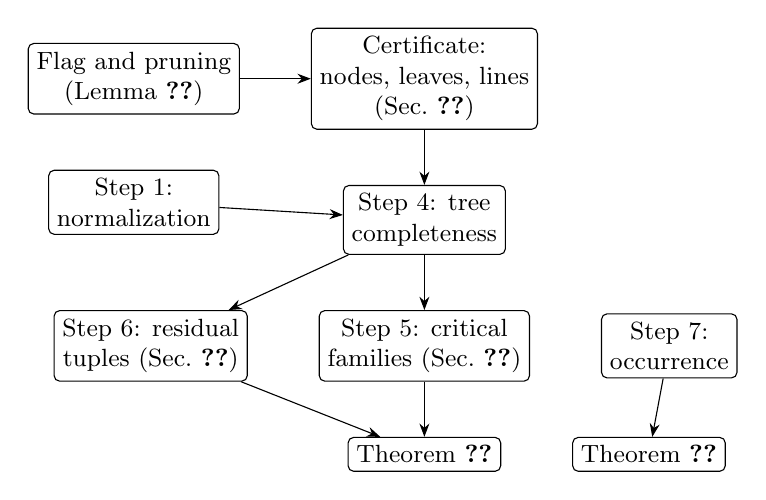
\begin{tikzpicture}[>=Stealth, node distance=7mm and 9mm, box/.style={draw, rounded corners=2pt, align=center, inner sep=3pt, font=\small}]
\node[box] (flag) {Flag and pruning\\(Lemma~\ref{lem:prune})};
\node[box, right=of flag] (cert) {Certificate:\\nodes, leaves, lines\\(Sec.~\ref{sec:cert})};
\node[box, below=of flag] (norm) {Step 1:\\normalization};
\node[box, below=of cert] (tree) {Step 4: tree\\completeness};
\node[box, below=of tree] (crit) {Step 5: critical\\families (Sec.~\ref{sec:tails})};
\node[box, left=of crit] (res) {Step 6: residual\\tuples (Sec.~\ref{sec:resid})};
\node[box, right=of crit] (occ) {Step 7:\\occurrence};
\node[box, below=of crit] (main) {Theorem~\ref{thm:main}};
\node[box, right=of main] (att) {Theorem~\ref{thm:attained}};
\draw[->] (flag) -- (cert);
\draw[->] (cert) -- (tree);
\draw[->] (norm) -- (tree);
\draw[->] (tree) -- (crit);
\draw[->] (tree) -- (res);
\draw[->] (crit) -- (main);
\draw[->] (res) -- (main);
\draw[->] (occ) -- (att);
\end{tikzpicture}
\caption{Dependencies of the macro-steps. An arrow from $X$ to $Y$ means that $Y$ uses $X$.}
\label{fig:dag}
\end{figure}

\begin{example}\label{ex:smallest}
The smallest case is $v=(1,2,3,4,5)$, $s=1$, with $\ML=1/6$. At $t=1/6$ the five distances are $1/6,1/3,1/2,1/3,1/6$, so $\ML\ge1/6$. For the upper bound see Example~\ref{ex:upper} below, which uses the tent-and-floor lemma of Section~\ref{sec:tails}. A tuple off both critical tori is $(1,3,4,5,7)$ with $\ML=2/11$: at $t=5/11$ the fractional parts of $t,3t,4t,5t,7t$ are $5/11,4/11,9/11,3/11,2/11$, so the distances are $5/11,4/11,2/11,3/11,2/11$ with minimum $2/11$. (In the families of Section~\ref{sec:tails} this tuple is $(V_2,5)$, and $2/11=s/(5s+1)$ for $s=2$.)
\end{example}

\section{The two critical families}\label{sec:tails}

This section proves Steps~5 and~7 of the outline. It needs only the definition of $\ML$. Its conclusions (Theorem~\ref{thm:crit}) are used in Section~\ref{sec:cert} to close the critical leaves. Everything in it is hand-written mathematics; the Lean statements are in the module \lean{ObsKS5Tail} (names given with each statement).

Let $V\in\{V_1,V_2\}=\{(1,2,3,4),(1,3,4,7)\}$. The critical torus is $U_V=\{(\alpha V,\beta)\}$ with $f=\min(f_V(\alpha),\dist\beta)$, where $f_V(\alpha)=\min_{v\in V}\dist{v\alpha}$. Since $\ML(V)=1/5$ (taking $\beta=1/2$), $M(U_V)=1/5$. Its primitive lines are $w=(AV,B)$ with $\gcd(A,B)=1$; since $\dist{-x}=\dist x$ we may take $A,B\ge1$. Write $G_V(t)=\min_{v\in V}\dist{vt}$ and $D(t)=\mathrm{dist}(t,\tfrac15\Z)$.

\begin{lemma}[$A\ge2$; Lean \lean{ML_ge_fifth_P}]\label{lem:P}
If $A\ge2$ then $\ML(w)\ge1/5$.
\end{lemma}
\begin{proof}
Let $t_h=(\tfrac15+h)/A$, $h=0,\dots,A-1$. The runners $Av_i$ sit at $v_i/5+v_ih\equiv v_i/5\pmod 1$, at distance $\ge1/5$ because $5\nmid v_i$. The last runner sits at $B/(5A)+Bh/A$, and $Bh$ runs over all residues modulo $A$ (since $\gcd(A,B)=1$), so some $h$ puts it within $1/(2A)$ of $1/2$, at distance at least $\tfrac12-\tfrac1{2A}\ge\tfrac14$.
\end{proof}
\begin{lemma}[$A=1$, $5\nmid B$; Lean \lean{ML_ge_fifth_N}]\label{lem:N}
$\ML(w)\ge1/5$.
\end{lemma}
\begin{proof}
At $t=1/5$ the runners sit at $v_i/5$ and $B/5$. None of the numerators is divisible by $5$, so each fractional part lies in $\{\tfrac15,\tfrac25,\tfrac35,\tfrac45\}$ and each distance is at least $1/5$.
\end{proof}
\begin{lemma}[witness; Lean \lean{ML_ge_V1}, \lean{ML_ge_V2}, \lean{ML_ge_V2_s1}]\label{lem:W}
For $s\ge1$ and $l=5s+1$, at $t=s/l$ the runners of $(V,5s)$ are at distances $s/l$ (speed $1$), $2s/l$ ($2$), at least $s/l$ ($3$), $(s+1)/l$ ($4$), $(2s-1)/l$ ($7$) and $s/l$ ($5s$). Hence $\ML(V,5s)\ge s/(5s+1)$; and $\ML(1,3,4,7,5)\ge2/11$ at $t=5/11$.
\end{lemma}
\begin{proof}
Direct. For example for speed $5s$: $5s\cdot s/l=s-s/l$ because $s\,l=5s^2+s$, so the distance is $s/l$. For speed $4$: $4s/l>1/2$ when $s\ge1$, so the distance is $1-4s/l=(s+1)/l$.
\end{proof}
\begin{lemma}[tent and floor; Lean \lean{lemmaH_V1}, \lean{lemmaH_V2}]\label{lem:H}
For all real $t$: $G_{V_1}(t)\le\max(\tfrac15-D(t),\tfrac17)$ and $G_{V_2}(t)\le\max(\tfrac15-D(t),\tfrac2{11})$. Both constants are attained: $G_{V_1}(2/7)=1/7$ with $D=3/35$, and $G_{V_2}(5/11)=2/11$ with $D=3/55$.
\end{lemma}
\begin{proof}
By evenness and periodicity take $t\in[0,\tfrac12]$. On each interval of the tables one runner's distance is an affine function of $t$ and the inequality is linear, so it suffices to check an endpoint.
\begin{center}\small
\begin{tabular}{ll}\toprule
$V_1$: interval & runner and condition\\\midrule
$[0,\frac15]$ & $\dist t=t\le\frac15-D$\\
$[\frac15,\frac14]$ & $\dist{4t}=1-4t\le\frac25-t$ iff $t\ge\frac15$\\
$[\frac14,\frac27]$ & $\dist{4t}=4t-1\le\frac17$ iff $t\le\frac27$\\
$[\frac27,\frac13]$ & $\dist{3t}=1-3t\le\frac17$ iff $t\ge\frac27$\\
$[\frac13,\frac25]$ & $\dist{3t}=3t-1\le t-\frac15$ iff $t\le\frac25$\\
$[\frac25,\frac12]$ & $\dist{2t}=1-2t\le\frac35-t$ iff $t\ge\frac25$\\\bottomrule
\end{tabular}
\qquad
\begin{tabular}{ll}\toprule
$V_2$: interval & runner and condition\\\midrule
$[0,\frac15]$ & as for $V_1$\\
$[\frac15,\frac14]$ & $\dist{4t}=1-4t\le\frac25-t$\\
$[\frac14,\frac7{25}]$ & $\dist{4t}=4t-1\le\frac25-t$\\
$[\frac4{15},\frac27]$ & $\dist{7t}=2-7t\le\frac25-t$\\
$[\frac27,\frac3{10}]$ & $\dist{7t}=7t-2\le\frac25-t$\\
$[\frac3{10},\frac13]$ & $\dist{3t}=1-3t\le t-\frac15$\\
$[\frac13,\frac25]$ & $\dist{3t}=3t-1\le t-\frac15$\\
$[\frac25,\frac37]$ & $\dist{7t}=3-7t\le\frac35-t$\\
$[\frac37,\frac7{15}]$ & $\min(7t-3,\,2-4t)\le\frac2{11}$ (crossing at $t=\frac5{11}$)\\
$[\frac7{15},\frac12]$ & $\dist{4t}=2-4t\le\frac35-t$\\\bottomrule
\end{tabular}
\end{center}
\end{proof}
\begin{proposition}[upper bound; Lean \lean{ML_le_of_tent}]\label{prop:U}
For $V\in\{V_1,V_2\}$, $p_V=\tfrac17,\tfrac2{11}$ respectively, and $s\ge1$: $\ML(V,5s)\le\max(\tfrac s{5s+1},p_V)$.
\end{proposition}
\begin{proof}
Let $d'=\max(\tfrac s{5s+1},p_V)$, let $t$ be arbitrary, $e\in\tfrac15\Z$ nearest to $t$ and $D=|t-e|$. Since $5se\in\Z$, $\dist{5st}\le5sD$. If $D\le d'/(5s)$ this is at most $d'$. Otherwise Lemma~\ref{lem:H} gives $G_V(t)\le\max(\tfrac15-\tfrac{d'}{5s},p_V)\le d'$, the last step being equivalent to $d'\ge s/(5s+1)$.
\end{proof}
\begin{theorem}[critical lines; Lean \lean{ML_V1_eq}, \lean{ML_V2_eq}, \lean{ML_V2_s1_eq}, \lean{thm1_i_A_ge_two}, \lean{thm1_i_A_one}]\label{thm:crit}
Let $w=(AV,B)$, $\gcd(A,B)=1$, $A,B\ge1$, with distinct entries. (i) If $A\ge2$, or $A=1$ and $5\nmid B$, then $\ML(w)\ge1/5$. (ii) If $A=1$ and $B=5s$ then $\ML(V_1,5s)=\tfrac s{5s+1}$ for $s\ge1$, $\ML(V_2,5s)=\tfrac s{5s+1}$ for $s\ge2$, and $\ML(1,3,4,5,7)=\tfrac2{11}$. In particular every near-tight line of a critical torus has value $s'/(5s'+1)$ for some $s'\ge1$.
\end{theorem}
\begin{proof}
(i) is Lemmas~\ref{lem:P} and~\ref{lem:N}. (ii) For $V_1$, $\tfrac s{5s+1}\ge\tfrac16>\tfrac17$, so Proposition~\ref{prop:U} and Lemma~\ref{lem:W} give equality. For $V_2$ and $s\ge2$, $\tfrac s{5s+1}\ge\tfrac2{11}$ iff $s\ge2$, again equality. For $s=1$ the upper bound is $\tfrac2{11}$ and the lower bound is Lemma~\ref{lem:W} at $t=5/11$; the value $2/11$ equals $s'/(5s'+1)$ with $s'=2$.
\end{proof}
Theorem~\ref{thm:attained} is the case $V=V_1$, $A=1$, $B=5s$ of part~(ii).

\begin{example}\label{ex:upper}
For $v=(1,2,3,4,5)$ ($V=V_1$, $s=1$): $d'=\max(\tfrac16,\tfrac17)=\tfrac16$, so $\ML\le\tfrac16$ by Proposition~\ref{prop:U}; with Lemma~\ref{lem:W} ($t=1/6$) this gives $\ML(1,2,3,4,5)=1/6$. Concretely, take $t$ with $D(t)=D$. The fifth runner has $\dist{5t}\le5D$, which is $\le1/6$ if $D\le1/30$; if $D>1/30$ then $\tfrac15-D<\tfrac15-\tfrac1{30}=\tfrac16$, so by Lemma~\ref{lem:H} the first four runners include one at distance $\le\max(\tfrac16,\tfrac17)=\tfrac16$.
\end{example}

\section{The tree: lattice lemmas and the case tree}\label{sec:tree}

This section proves Steps~1 and~2 of the outline and states what Step~4 asks of the certificate. It needs the notation of Section~\ref{sec:notation}. Its output (the case tree, Section~\ref{sec:cert}) is consumed by the certificate and by Section~\ref{sec:resid}. The geometry is the same as in the four-speed case: only the number of rows (four instead of three) and the threshold ($1/5$ instead of $1/4$) change. The lemmas below are stated in the form needed for rank four; the Lean modules are \lean{L5S3.*} (flag geometry, Babai rounding, greedy existence) and \lean{L5S4.*} (tree induction, symmetry). The exact hypotheses of every Lean statement have not been compared line by line with the statements below (Section~\ref{sec:limits}).

\paragraph{Normalization (Step 1).} Let $v\in\Z^5$ have positive pairwise distinct entries and $\ML(v)<1/5$. Write $v=gw$ with $g\ge1$ and $w$ primitive; $\ML(v)=\ML(w)$ (substitute $t\mapsto t/g$, a bijection of $\R$ onto itself). Replacing $w$ by $\sigma w$ for $\sigma\in\mathrm{SP}$ does not change $\ML$; so it is enough to treat primitive $w$ with nonzero entries and pairwise distinct absolute values and $\ML(w)<1/5$. (Lean: \lean{exists_prim5}, \lean{nf_ML_smul}, \lean{ML_act}.) Distinctness of the absolute values is used only in the line check (Section~\ref{sec:cert}), where lines with a repeated absolute entry are not examined; the pruning lemma does not need it. This is why the Lean statement can be proved for injective $v$ without discussing repeated speeds.

\begin{lemma}[greedy flags; Lean \lean{flag_exists}, \lean{greedyBasis_exists}]\label{lem:flag}
Every primitive $v\in\Z^5$ has a greedy flag $(h_0,h_1,h_2,h_3)$; it is a $\Z$-basis of $\Lambda$, each initial segment spans a saturated sublattice, and the matrix $H$ with rows $h_i$ has an integer right inverse.
\end{lemma}
\emph{Proof sketch.} By induction on the number of rows chosen, with the statement that the rows chosen so far are rationally independent, greedy at each step, and saturated in $\Lambda$. A candidate exists because $\Lambda$ has rational dimension four. The next row minimizes a positive integer (a Gram determinant). Saturation follows from a shear identity: if $x\in\Lambda$ lies in the rational span of $h_0,\dots,h_i$ with coefficient $\lambda$ on $h_i$, replacing $x$ by $x-eh_i$ with $e$ nearest to $\lambda$ multiplies the Gram determinant by $(\lambda-e)^2\le\frac14$, which contradicts minimality unless $\lambda=e$. The right inverse comes from the primitivity of $v$.

\begin{lemma}[pruning; Lean \lean{L5S3.ratio34_thm}, \lean{stage_dist_thm}, \lean{ML_ge_of_close}, \lean{stage_prune}, \lean{node_of_stage}]\label{lem:prune}
Let $v\in\Z^5$ be primitive with nonzero entries and $\ML(v)<1/5$, and let $(h_0,\dots,h_3)$ be a greedy flag. Then:
\begin{enumerate}
\item[(a)] (ratio) $\mu_{i+1}^2\ge\tfrac34\mu_i^2$ for $i=1,2,3$.
\item[(b)] (stage bound) for every $k\in\{0,\dots,3\}$, every $x\in T(L_k)$ with $f(x)\ge c\ge1/5$,
\[
4\bigl(c-\tfrac15\bigr)^2<\sum_{k<i\le4}\mu_i^{-2}.
\]
\end{enumerate}
\end{lemma}
\emph{Proof.} (a) Let $h^*_i$ be the Gram--Schmidt vector of $h_i$, $\lambda$ the coefficient of $h_{i+1}$ on $h^*_i$ and $e$ the integer nearest to $\lambda$; the vector $u=h_{i+1}-eh_i\in\Lambda$ has component orthogonal to $h_0,\dots,h_{i-1}$ of squared norm $\mu_{i+2}^2+(\lambda-e)^2\mu_{i+1}^2\le\mu_{i+2}^2+\tfrac14\mu_{i+1}^2$. Greediness of $h_i$ gives $\mu_{i+1}^2\le$ this, which is (a).

(b) \emph{Nearest plane.} Put $p=Hx$; $p_i\in\Z$ for $i<k$. Let $H H^{\top}=LDL^{\top}$ be the Gram--Schmidt factorization ($D=\mathrm{diag}(\mu_i^2)$). Choose integers $a_i$ and reals $w_i$ one after the other so that $p-a=Lw$ and $|w_i|\le\tfrac12$; for $i<k$ one gets $w_i=0$. Then $\sum_iw_i^2/\mu_{i+1}^2\le\tfrac14\sum_{i\ge k}\mu_{i+1}^{-2}$. \emph{From the plane to the line.} With $y=x-Ra$ ($R$ the integer right inverse), $H(y-s)=0$ for $s=H^{\top}L^{-\top}(w/D)$, and $\ker H=\R v$, so $x-z-tv=s$ with $z\in\Z^5$, $t\in\R$ and $|s|^2=\sum_iw_i^2/\mu_{i+1}^2$. \emph{Loneliness.} Each coordinate of $s$ is at most $\rho=\tfrac12(\sum_{i>k}\mu_i^{-2})^{1/2}$, and $\dist{\cdot}$ is $1$-Lipschitz and $1$-periodic, so $\dist{tv_j}\ge\dist{x_j}-\rho$ for every $j$, i.e.\ $\ML(v)\ge f(x)-\rho$. With $\ML(v)<1/5\le c\le f(x)$ this is the claim. $\square$

The same inequalities, with the same proof, hold with $4$ in place of $5$ in the threshold and rank three. The consequence used by the certificate is obtained by splitting the sum in (b) at the depth $d$ and bounding the tail by (a): $\sum_{d\le i\le4}\mu_i^{-2}\le C_d\mu_d^{-2}$ with $C_d=\sum_{s<5-d}(4/3)^s$. In the five-speed tree the stage bound is applied at every earlier stage, not only at the expanding step; this is what makes the tree small enough to certify, and the resulting multi-stage statement and the lower bound on $\mu_4$ in terms of the leaf are in the \lean{L5S3} and \lean{L5S4} modules.

\paragraph{The case tree.} Using Lemma~\ref{lem:prune} one proves, by induction on the depth, that a near-tight primitive $v$ has a greedy flag whose first $d$ rows form a node of the following kind.
\begin{itemize}
\item \emph{Depth one.} $h_0$ is a primitive vector with entries in $[0,4]$ up to signed permutation and $2\le|h_0|^2\le18$ (the test of Lemma~\ref{lem:prune}(b) at the point $(\tfrac12,\dots,\tfrac12)$ bounds $|h_0|^2$). There are $26$ such vectors up to $\mathrm{SP}$ (Lean: \lean{d1_t1}).
\item \emph{Depth two.} $h_1$ modulo $\Z h_0$ is a class $\tau\in\Z^4$ in an explicit box determined by a witness point of $T(L_1)$ with loneliness $>1/5$; filters (gcd, coordinate vectors, ratio, stage bounds) keep a subset of the box. Signed permutations that fix $h_0$ identify equivalent nodes; the certificate keeps one representative per class.
\item \emph{Depth three (leaves).} For each representative, $h_2$ ranges over a window determined by a witness point of $T(L_2)$; the filters again apply. The leaf records store, for each leaf, a witness point of $T(L_3)$ (its loneliness $c_3\ge1/5$) and a basis of the plane $\Gamma$.
\item \emph{Lines.} For a leaf with $c_3>1/5$ the last row gives a window for $|v|^2$ (from the ratio test at $i=4$ and the stage bounds at $d=4$), and $v$ lies in $\Gamma$. A class of leaves with the same plane up to $\mathrm{SP}$ carries one table of lines. Every line in the window is either closed by a time ($\ML\ge1/5$), or is excused (not primitive, a zero entry, two equal absolute entries), or is a signed permutation of one of the residual tuples.
\item \emph{Critical leaves.} If $c_3=1/5$ is the best witness the window is unbounded; these are the leaves where $\Gamma$ is, up to $\mathrm{SP}$, $\langle(V,0),e_5\rangle$ with squared covolume $30$ ($V_1$) or $75$ ($V_2$). There are $8$ of them, all below one representative of depth two (number $304$ in our numbering), in two classes.
\end{itemize}
This yields Step~4: \emph{every primitive $v\in\Z^5$ with nonzero pairwise distinct absolute entries and $\ML(v)<1/5$ is, up to $\mathrm{SP}$, either a line $(AV,B)$ of a critical torus or one of $25$ residual tuples}. (Lean: the stream hypothesis \lean{StreamHyp'} and the theorem \lean{tree_complete_unconditional'}, with its hypotheses discharged by the aggregation of Section~\ref{sec:cert}.) The residual tuples are those lines that are not closed by a time and not on a critical torus; Section~\ref{sec:resid}.

\section{The certificate}\label{sec:cert}

This section describes what the generated data are, how they are assembled so that the Lean kernel can check them, and their size. It uses Lemma~\ref{lem:prune} and the case tree of Section~\ref{sec:tree}; Section~\ref{sec:trust} uses it. All counts in this section are facts about generated data, computed by the generators and recounted by independent code where stated; they are not Lean theorems, and no theorem depends on their being as printed, except where a figure is marked as proved by \lean{decide +kernel}.

\begin{table}[ht]
\centering\small
\begin{tabular}{lrp{5.6cm}}
\toprule
object & count & remark\\
\midrule
depth-one nodes & $26$ & three of them carry no representative\\
depth-two nodes before pruning & $67{,}012$ & unpruned search\\
depth-two nodes surviving the multi-stage pruning & $30{,}649$ & \\
representatives of depth-two nodes under $\mathrm{SP}$ & $1{,}965$ & block sizes per depth-one node sum to $1{,}965$ \\
leaf records & $693{,}222$ & \\
leaf classes (lines tables) & $81{,}436$ & \lean{lines_count} proves this by \lean{decide +kernel} with no axioms\\
critical leaves & $8$ & all under one representative, two classes\\
lines & $9{,}593{,}060$ & $6{,}151{,}393$ distinct tuples\\
residual tuples & $25$ & entries at most $35$\\
\bottomrule
\end{tabular}
\caption{The certificate in numbers (output of the generators, recounted by independent code in several cases).}
\label{tab:funnel}
\end{table}
For comparison, the first, unpruned computation of the tree (not used in the Lean proof) had $20{,}194{,}818$ leaves and $13.19\times10^9$ line checks with minimum margin $1/45$; a second program re-enumerated every depth-two node and every leaf and matched, and an independent exhaustive search of all $2{,}450{,}913{,}356$ primitive quintuples with largest speed at most $200$ found exactly the $92$ near-tight quintuples of the tree's output.
These checks corroborate the generators; they are not part of the proof.

\subsection{Leaf rollout}\label{sec:rollout}

The data for one representative of depth two (its leaf records, the stored class tables of its leaves, and the proof that every leaf passes the leaf test) form a small group of generated Lean modules. A driver script builds the modules of one representative at a time under a memory ceiling and records the result. Every one of the $1{,}965$ representatives has a result row: $1{,}957$ were built by the driver, and $8$ were built earlier by separate chains (the two largest, number $265$ with $23{,}228$ leaves and number $304$ with $18{,}520$ leaves and the eight critical leaves, and six small ones).
For each critical leaf the leaf test is replaced by an identification record: an index in $\{0,1\}$ for the critical torus, a signed permutation, and two $2\times2$ integer matrices, and the kernel checks that the plane of the leaf maps onto $\langle(V,0),e_5\rangle$ (Lean \lean{crit_linkW}, \lean{d3Crit_leafRel}; the value $\ML$ on that torus is then Theorem~\ref{thm:crit}).

\subsection{Lines: the row-interval checker}\label{sec:lines}

A leaf class has a plane $\Gamma$ with a reduced basis $k_0,k_1$ and Gram entries $(a,b,c)$, $D=ac-b^2$ (squared covolume). A line is $u=xk_0+yk_1$ and $|u|^2=n$ satisfies the identity $a\,n=(ax+by)^2+Dy^2$. The window gives $lo\le n\le hi$. The earlier checker visited every integer point of a box. The checker that is used stores, for every row $y=1,\dots,Y$, four integers $p,g_1,g_2,r$ such that $x\le p$ or $x\ge r$ forces $n>hi$ and $g_1\le x\le g_2$ (a hole, possibly empty) forces $n<lo$, each verified by two inequalities from the identity; the kernel then walks only the segments $p+1,\dots,g_1-1$ and $g_2+1,\dots,r-1$. Each visited point reads one stored hint of $11$ bits: a time $a/q$ from a fixed list (checked directly, no search), or an excuse (not primitive, a zero entry, two equal absolute entries, one of the residual tuples, out of range). The soundness theorem is \lean{classLinesR_sound}: if the checker accepts a class then every primitive $u$ in the class with nonzero pairwise distinct absolute entries has a residual tuple up to $\mathrm{SP}$ or $\ML(u)\ge1/5$. The recorded figures: $1{,}045{,}372$ rows, $15{,}352{,}485$ visited points, $9{,}593{,}060$ lines, a certificate of $235{,}781{,}143$ bits and a largest class of $116{,}941$ bits; an independent Rust regeneration written from the mathematical statement, without reading the prototype, agrees with all aggregates, and a brute-force scan of the old box over all $81{,}436$ classes ($82{,}439{,}308$ points) found no point that the checker misses.
Two points about this stage must be stated. First, the checker is applied per class, not per leaf; so a leaf's lines are covered only if the leaf is registered to its class (next subsection). Second, the times come from one fixed table of $548$ reduced fractions $a/q$ with $5\le q\le60$ and $1\le a\le q/2$ (the Lean definition \lean{TL5}); a time listed for a point is checked directly, without search.

\subsection{Registration by signed-permutation advice}\label{sec:reg}

The leaf records of a representative carry their own local class tables, and the lines stage is stored once per class. To connect them, an exact match of rows is not available (the local class rows are the Hermite normal form of $G\cdot l$ for a signed permutation $G$ while the lines records store $l$ before $G$). The registration therefore transfers the lines clause along a signed permutation: for each local class a Rust generator finds the matching lines record and an integer matrix $M$, supplied as \emph{advice}; the kernel checks that $M$ does what is claimed (Lean \lean{linesCl_transfer}, \lean{eqChk_sound}, \lean{linesLoc_of_adv}, in \lean{L5Reg.Equiv}, $165$ lines; one \lean{Reg<c>} module per representative).
Wrong advice is rejected: controls with a wrong offset, a dropped entry and a perturbed matrix make the check fail. For the two largest representatives the check is split into parts of $100$ classes.

\subsection{Aggregation: a fan-in tree}\label{sec:agg}

The statement the tree needs is a single clause over all $1{,}965$ representatives. Importing roughly $10{,}000$ generated modules into one module is impractical, so the representatives are combined by a tree of small modules: a \emph{block} is a size, an accessor for the node of each representative, and the concatenation of the local class tables; the only combinator is \lean{append}, and a master appends at most eight blocks. The final tree has $258$ leaf masters, $32$ middle masters, $23$ roots (one per non-empty depth-one node: $26$ minus the three empty ones) and a top module \lean{AggFive.Top}. A mirror tree of $314$ modules (\lean{AggFive.Hl}: $258+32+23+1$) carries the lines clause for each representative.
The top theorem \lean{five_speed_spectrum2} is stated under a hypothesis \lean{FiveSpeedHyps2}, which consists of a structure \lean{Top.Holes} (one field per representative whose module was not yet built, a device that allowed the aggregation to be assembled before every representative was finished) and a tree of propositions \lean{HLines}. Now that every representative is built, both are trivial: \lean{Top.Holes} is a structure with no field, and every structure in the \lean{HLines} tree has no field (checked by a script over all $258$ leaf structures). The module \lean{FiveSpeedFinal3} states this: \lean{hyps2_trivial} instantiates the hypothesis with the empty structure and \lean{repeat' constructor}, and \lean{five_speed_spectrum_final} is \lean{five_speed_spectrum2} applied to it. The real content lies in the proofs of the representatives' own theorems in the leaf modules, such as \lean{lines219}; these are checked by the kernel but are not individually discussed here.

\section{Residual tuples}\label{sec:resid}

This section closes the $25$ residual tuples. It uses Section~\ref{sec:cert}; the theorem of Section~\ref{sec:intro} uses it. The residual tuples are the sorted quintuples that the line check sets aside because no time closes them; they have entries at most $35$. An earlier, independent Lean theorem (module \lean{L5WP1}, \lean{box30_unordered}, \lean{box45_unordered}, \lean{box60_unordered}) states, for five pairwise distinct positive integers at most $B\in\{30,45,60\}$, that $\ML<1/5$ holds exactly when a rearrangement is a positive multiple of a tuple of a stored list and then $\ML=s/(5s+1)$; the proof is a kernel evaluation of witness times over all sorted tuples up to $B$. Since all residual tuples have entries at most $45$, their values are given by \lean{box45}; no new data is needed.
The mathematical content of the list, as computed (not a Lean statement): the primitive near-tight quintuples are, up to signed permutation, $(1,2,3,4,5s)$ ($s\ge1$), $(1,3,4,7,5s)$ ($s\ge2$), $(1,3,4,5,7)$, and twelve sporadic tuples $(1,2,3,5,8)$ [$2/11$], $(1,3,4,5,9)$ [$1/6$], $(1,3,4,5,11)$ [$3/16$], $(1,3,4,5,18)$ [$2/11$], $(1,3,4,5,27)$ [$6/31$], $(1,4,5,6,7)$ [$2/11$], $(1,4,5,6,27)$ [$6/31$], $(1,7,8,9,15)$ [$3/16$], $(2,3,5,8,19)$ [$4/21$], $(2,5,7,8,9)$ [$3/16$], $(3,5,8,9,13)$ [$4/21$], $(3,5,8,11,13)$ [$4/21$].
Each of these values is $s/(5s+1)$ for some $s\ge1$. The twelve tuples and their values coincide with the list of near-tight quintuples off both critical tori in Cordella~\cite{Cordella}, Section~6.2, compared item by item; what the present proof adds is that there are no others.

\section{Trust base}\label{sec:trust}

This section lists what a reader must accept in order to accept Theorem~\ref{thm:main}, and what the paper does not rely on. It uses the statements of Section~\ref{sec:intro} and the certificate of Section~\ref{sec:cert}; Section~\ref{sec:repro} gives the means to check the items.

\begin{enumerate}
\item The Lean~4 kernel (toolchain \lean{leanprover/lean4:v4.30.0}) and Mathlib~\cite{Mathlib} at the revision pinned in \lean{lake-manifest.json} (\lean{c5ea00351c28e24afc9f0f84379aa41082b1188f}).
\item The definition of $\ML$ in the module \lean{MaxLoneliness}, exactly as follows. The reader should compare it with the statement of Theorem~\ref{thm:main}.
\VerbatimInput[fontsize=\footnotesize,frame=single,framesep=2mm]{snippets/nid_def.lean}
\VerbatimInput[fontsize=\footnotesize,frame=single,framesep=2mm]{snippets/gap_def.lean}
\VerbatimInput[fontsize=\footnotesize,frame=single,framesep=2mm]{snippets/ml_def.lean}
Here \lean{gap v t} is $\min_i\dist{tv_i}$ with $t$ real; the range of \lean{gap v} is nonempty and bounded above by $1/2$ (\lean{bddAbove_range_gap}), so \lean{sSup} is a genuine supremum and no junk value can occur; the paper writes $\max$, and for integer speeds the supremum is attained (a fact that is not needed and not stated in Lean).
\item Axioms: the script \texttt{check\_axioms.sh} of the repository prints \texttt{\#print axioms} for the headline theorems and judges the output. For \lean{five_speed_spectrum_final}, \lean{five_speed_spectrum_iff_final} and \lean{five_speed_attained} it prints exactly \lean{propext, Classical.choice, Quot.sound}. Two deliberately planted control theorems (one directly proved by \lean{sorry}, one transitively) print \lean{sorryAx}, which shows that the instrument sees a \lean{sorry}. The recorded output is in \texttt{repro/expected\_output/}.
\item Source scans. A scan of the $17{,}598$ modules of the import closure of \lean{FiveSpeedFinal4}, with comments removed (script \texttt{source\_scan.sh}), finds no \lean{sorry}, \lean{native_decide}, \lean{axiom}, \lean{unsafe}, \lean{implemented_by}, \lean{extern}, \lean{opaque} or \lean{ofReduceBool}; \lean{Classical.choose} occurs on two lines of one file, and \lean{decide +kernel} on $49{,}948$ lines. A text search for \lean{sorry} in the whole development tree additionally finds $48$ files that contain planted control theorems (corrupted records, wrong advice, a planted \lean{sorry}), used to check that the instruments detect failures. None of these $48$ files is in the import closure of the headline theorem: the headline modules import the clean mirror modules \lean{AggFive.Clean.*}, and the $48$ files are not part of the repository's \texttt{lean/} directory. Their list is in \texttt{repro/expected\_output/planted\_controls.txt}; a plan for moving them out of the library modules that contain them is in \texttt{repro/PROPOSAL\_MOVE\_CONTROLS.md} and has not been carried out.
\end{enumerate}
The Rust generators are not in the trust base: they produce certificates that the kernel checks against definitions whose soundness theorems are proved in Lean. A wrong certificate can make a kernel check fail but cannot prove a false statement.

\paragraph{The statements, copied from the source files.}
\VerbatimInput[fontsize=\footnotesize,frame=single,framesep=2mm,label={FiveSpeedFinal3.lean, lines 20--22}]{snippets/final3_stmt.lean}
\VerbatimInput[fontsize=\footnotesize,frame=single,framesep=2mm,label={FiveSpeedFinal4.lean, lines 14--16 (statement; the proof follows in the file)}]{snippets/final4_stmt.lean}
\VerbatimInput[fontsize=\footnotesize,frame=single,framesep=2mm,label={FiveSpeedOfTree.lean, lines 269--270}]{snippets/attained_stmt.lean}
The first two are in namespace \lean{LRSpectrumFull.L5S5} (the file \lean{FiveSpeedFinal3} imports the conditional theorem \lean{five_speed_spectrum2} and applies it to the trivial instance of its hypothesis; there is no further hypothesis). Casts of integers to reals are implicit in the typeset reading of the statements: ``five distinct positive integer speeds'' is an injective function $v:\{0,\dots,4\}\to\Z$ with positive values, and $\ML(v)<1/5$ is a real inequality.

\subsection{What the kernel check guarantees and what it does not}\label{sec:guarantee}

\emph{What the kernel guarantees.} (1) The proof term of each headline theorem has the type stated above and depends only on the three standard axioms. (2) The generated data are not trusted. A data module is a list of integer records; the kernel evaluates a Boolean function of the list and accepts the theorem \lean{check data = true} only if it reduces to \lean{true}. The meaning of that statement is fixed by soundness theorems proved in Lean (for the lines stage \lean{classLinesR_sound}, for the registration \lean{linesLoc_of_adv}). A wrong record, a missing leaf or a missing line makes some test false and the build fails; it cannot produce a false theorem.

\emph{What it does not guarantee.}
\begin{itemize}
\item That the Lean statement is the mathematical statement the reader has in mind; this is a matter of reading the definitions above. No human expert has yet done this reading for the present release.
\item That the soundness theorems, the Boolean checkers and the lemma statements say what Sections~\ref{sec:tree} and~\ref{sec:cert} say they say. They are kernel-checked as Lean statements; whether the lemma statements of this paper are the Lean statements is a matter of reading, and has not been checked line by line.
\item The counts of Table~\ref{tab:funnel} and of the other figures: they are generator facts, recounted by independent code in several cases, not Lean theorems (except \lean{lines_count}).
\item Absence of vacuity. A checker could be too weak. The planted controls (corrupted records, wrong advice, a planted \lean{sorry}) are evidence against vacuity, not a proof of it. The theorems \lean{L5Reg.lines<c>} of the individual representatives and the mapping performed by the generators have not been audited individually; only their axiom prints are known.
\item That the mathematical statement is true outside Lean. If the Lean definition of $\ML$ is the standard one, the kernel check is a proof of the standard statement; truth outside Lean rests on that identification and on the trust items above. No human has independently checked the tree and the line tables.
\end{itemize}

\section{Limitations}\label{sec:limits}

\begin{itemize}
\item \emph{No human review.} The kernel checks every formal step. No human has read the whole argument, the generators or the line tables, and the paper does not claim that anyone has. An independent mathematical review of the tree and of the line tables has not been carried out.
\item \emph{Statements.} The lemma statements in Section~\ref{sec:tree} are written in the form we believe the Lean modules prove; they were not compared hypothesis by hypothesis with every Lean declaration. A reader who needs the exact statements should read the Lean files (Appendix~A).
\item \emph{Planted controls.} Planted-\lean{sorry} control theorems live in library modules of the development tree that are not imported by the headline theorem and are not part of the repository; moving them to modules that nothing imports is proposed but not done (Section~\ref{sec:trust}).
\item \emph{Reproduction.} No clean rebuild from scratch was run: the proof was built incrementally, with restarts. The regeneration of the generated data is partial (Section~\ref{sec:repro}), and the sources of the generators contain a placeholder path prefix that the regeneration script replaces in working copies.
\item \emph{Scope of the claim of priority.} The searches behind Section~\ref{sec:prior} are dated and have gaps. For five speeds, the last full reading of the literature was on 15 November 2026 and the last repetition of a search on 17 November 2026.
\end{itemize}

\section{Reproducibility}\label{sec:repro}

This section says what is provided for rebuilding the proof; nothing else in the paper uses it. The commands are in the directory \texttt{repro/} of the accompanying repository, and its \texttt{README.md} gives the three-command route.

\paragraph{Entry points.} The headline modules are \lean{FiveSpeedFinal3} and \lean{FiveSpeedFinal4} in the namespace \lean{LRSpectrumFull.L5S5}. They are built with \lean{lake build} on one module at a time, never with a whole-tree build: \texttt{lake} starts one Lean worker per core by default, and one worker for this project needs between about $4$ and $10$ GB. The build of \lean{FiveSpeedFinal4} reports $20{,}192$ jobs; a replay with \lean{lake build --no-build} on an already built tree peaks at about $780$ MB. The generators are Rust programs (\lean{l5s4o} for class tables, \lean{l5_reg} for registration advice, \lean{l5lines_emit} for the row-interval records, \lean{l5v3} for the leaf data, \lean{l5_agg} for the aggregation and \lean{l5hlines} for its mirror). The shell drivers that built the tree one representative or one chunk at a time under a memory ceiling are shipped as documentation only.

\paragraph{Contents and observed results.} The repository contains a manifest, a build script, an axiom-check script, a regeneration script, the Rust sources of the generators and the input tables. Of the $17{,}598$ modules of the import closure, $9{,}496$ are shipped, among them \lean{GD3O1} and the $183$ \lean{GD3O*} modules of eight representatives (numbers $265$, $304$, $927$, $1075$, $1336$, $1343$, $1524$, $1763$) that the generators do not reproduce byte for byte; the other $8{,}102$ (the families \lean{GD3O*} and \lean{LinRQSC*}, $635.1$ MB) are listed with their sha256 values and are restored by the regeneration script. The following results were observed on the development tree, which had been built incrementally.
\begin{itemize}
\item \emph{Manifest.} The import closure of \lean{FiveSpeedFinal4} has $17{,}598$ project modules with $707.9$ MB of Lean source. The manifest lists them in import order with a sha256 value and the generating program of each. The build script (\texttt{build.sh}) builds one module per \lean{lake} call, with a memory gate, and can be resumed.
\item \emph{Replay.} \lean{lake build --no-build} on \lean{FiveSpeedFinal4} reports that all targets are up to date ($20{,}192$ jobs).
\item \emph{Axioms.} The axiom-check script printed seven lines, all as expected (PASS, $7$ of $7$): \lean{five_speed_spectrum_final}, \lean{five_speed_spectrum_iff_final}, \lean{five_speed_attained} and \lean{five_speed_spectrum2} depend on \lean{propext}, \lean{Classical.choice}, \lean{Quot.sound} only; \lean{hyps2_trivial} depends on no axiom; two planted controls report \lean{sorryAx}, as they must.
\item \emph{Source scan.} A scan of the $17{,}598$ closure modules, comments removed, found no \lean{sorry}, \lean{native_decide}, \lean{axiom}, \lean{unsafe} or \lean{ofReduceBool}.
\item \emph{Regeneration.} \texttt{regen\_data.sh --full} regenerated $19{,}614$ files from the Rust sources and found them byte-identical to the corresponding files of the development tree ($0$ different; $5$ files had no reference because they lie outside the closure). Covered: all $1{,}053$ \lean{LinRQSC*} modules; the node and blob families of \lean{GD3N*}, \lean{GD3F2N*} and \lean{GD3F2L*}; $7{,}051$ of the $7{,}233$ \lean{GD3O*} modules; the \lean{Reg*} modules and their memory files for five representatives only; the whole of \lean{AggFive} and all $314$ modules of \lean{AggFive.Hl}.
\end{itemize}
A rebuild from scratch is estimated at about $36.8$ hours of Lean time (a cost-model figure, one process at a time) plus the regeneration of the omitted modules.

\paragraph{What was not done.} \emph{There is no clean-rebuild claim.} No from-scratch rebuild was run; the development tree was built incrementally, with restarts. The regeneration is partial: the \lean{Reg*} modules were regenerated for $5$ representatives only; eight representatives (the two largest, numbers $265$ and $304$, and six others built by an earlier chain) and several families were not regenerated, and a rerun of \lean{l5s4o} on those eight gives different files, which is why their modules are shipped as files; the class tables of the fourth step are copied inputs, not regenerated. The generator sources contain a placeholder path prefix, which the regeneration script replaces in working copies. The figures in this section are for incremental builds.

\section{Prior art}\label{sec:prior}

This section says what is known, what we take from it and what we do not claim. It uses the statements of Section~\ref{sec:intro}; nothing uses it. Statements about other papers refer to the versions cited in the bibliography.

\paragraph{Four speeds and the method.} Yi, Gill and Bu~\cite{YGB} prove the four-speed spectrum (their Theorems~1.1 and~1.2: the values below $1/4$ are exactly $m/(4m+2)$, $m\ge2$, $m\ne3$) by a density lemma and an exact search over $800{,}816{,}099$ quadruples, in C and Python, with no proof assistant. The architecture of a reduction through successive minima of the relation lattice, two critical subtori, and a finite exact search is theirs; the present proof follows the same overall shape. Jain and Kravitz~\cite{JK} proved the four-speed spectrum up to a finite set of undetermined exceptions, and Fan and Sun~\cite{FanSun} conjectured it (Conjecture~4.1).

\paragraph{Five speeds.} \emph{Yi, Gill and Bu.} In arXiv:2610.40694v1 (28 October 2026), their Theorem~1.7 (equal to Theorem~11.5) says that every coordinate-free $2$-dimensional subtorus of $(\R/\Z)^5$ with $\ML<2/9$ is $T(1,2,3,4)\times T$ or $T(1,3,4,7)\times T$ (value $1/5$), and that the only accumulation point of the five-speed spectrum below $2/9$ is $1/5$; their Corollary~11.6(ii) says that a primitive quintuple with $\ML<1/5$ and $|v|\ge33{,}750$ is of the form $\{a,2a,3a,4a,b\}$ or $\{a,3a,4a,7a,b\}$. They do not treat the values on the lines for $n=5$, do not list the near-tight quintuples below $33{,}750$ and do not claim a run of that finite set (about $6\times10^{19}$ sorted tuples). Consistently with their threshold, no tuple in our final list has norm near $33{,}750$; the largest off-torus tuple is $(1,4,5,6,27)$, with $|v|\approx28.4$.
\emph{Cordella.} Cordella~\cite{Cordella} gives the exact values on the two critical families (Theorem~4.2), reports that the exceptional set of the five-speed spectrum is finite but does not determine it (Theorem~6.4), and lists in Section~6.2 the $64$ primitive near-tight quintuples with speeds at most $130$, $52$ on the two critical tori and $12$ on neither.
Our twelve tuples and their values agree with that list item by item. The value on the first critical family is due to Kravitz~\cite{Kravitz21}. \emph{What remains ours:} the proof that the two families and these twelve tuples (with the tuple $(1,3,4,5,7)$ on the second family) are all, the value set $\{s/(5s+1)\}$, and the kernel check of all of it.
\emph{Other.} Oliner~\cite{Oliner} (Zenodo, November 2026; according to its record, machine-generated and not refereed) cites Yi--Gill--Bu; according to the theorem headers we read in its supplement (not built), it contains Lean statements of the exact values of families of four and five speeds, and a conditional statement that certain quintuples have $\ML\ge1/5$; we found no statement of the five-speed spectrum below $1/5$ in it, and we make no statement about the correctness of those files. Chen~\cite{Chen} formalizes the lonely runner conjecture for three to seven runners; the repository contains no spectrum statement that we found. The statement tracker~\cite{FC} contains the lonely runner conjecture and a variant of Tao, not a spectrum.

\paragraph{What we do not claim.} We do not claim that the five-speed statement was open as a mathematical question before this work, nor that it has no published proof; we claim a complete kernel-checked proof. We do not claim the framework (due in its essentials to~\cite{YGB} and the earlier work cited above). To our knowledge, as of the searches of 15 and 17 November 2026, we do not know of another complete proof of the five-speed spectrum, on paper or formal. That sentence is dated; a later reader should re-evaluate it against the literature.

\paragraph{The searches.} On 15 November 2026 we searched OpenAlex, arXiv, Zenodo, and GitHub repositories, issues and pull requests, and read~\cite{YGB} in full; on 17 November we repeated searches of Zenodo, GitHub, arXiv, the formal-conjectures repository, the Lean Zulip archive and the general web for formalizations of the four-speed spectrum and related statements. These searches have limits: two search engines did not return~\cite{YGB} itself on some queries; code search on large repositories is incomplete; the Lean Zulip index stops in February 2026; Google Scholar, zbMATH and MathSciNet were not reachable; a private effort would be invisible. No arXiv paper after 28 October 2026 that proves or supersedes the five-speed statement was found in the indexed window. No search specific to the five-speed statement was made after 17 November 2026.

\section{Provenance}\label{sec:prov}

The Lean modules, the Rust certificate generators and checkers, and the first draft of this paper were produced by an AI system (Claude, Anthropic); fresh sessions of the same system reviewed them; the questions, the research directions and the decision to formalize this statement came from Vico Bonfioli. The Lean kernel, not a human referee, checks the proofs.

\appendix
\section{Lean modules}
This appendix lists the Lean modules of the proof by group, for readers who rebuild it (Section~\ref{sec:repro}); it is not used by the mathematical argument. All modules are in namespace \lean{LRSpectrumFull}. File counts for \lean{L5S4}, \lean{L5Reg} and \lean{AggFive} are the numbers of modules in the import closure of \lean{FiveSpeedFinal4} (the closure has $17{,}598$ project modules), not of the whole directories; the other counts are from a directory listing of the development tree.
\begin{center}
\begin{tabular}{llp{8.2cm}}
\toprule
group & files & content\\
\midrule
\lean{ObsKS5Tail} & 1 & Section~\ref{sec:tails}: tent and floor, witnesses, critical-line values\\
\lean{L5WP1} & many & box theorems for speeds up to $30,45,60$ (residual tuples)\\
\lean{L5S3} & 18 & flag geometry: Gram matrices, greedy basis, Babai rounding, pruning\\
\lean{L5S4} & 14{,}320 & tree induction, symmetry transport (\lean{Sym}, \lean{ChainRep}, \lean{Records}), depth-two data, leaf records and chunks, line checker (\lean{LinRCore}, \lean{LinRSound}, \lean{LinRGlue}), and the generated data\\
\lean{L5Reg} & 2{,}446 & registration modules \lean{Reg<c>} and the transfer lemma \lean{Equiv}\\
\lean{AggFive} & 337 & aggregation tree (258 leaf, 32 mid, 23 root masters, \lean{Top}); in the closure also \lean{AggFive.Clean} ($54$) and the mirror \lean{AggFive.Hl} ($314$), counted separately\\
\lean{L5S5} & 14 & \lean{FiveSpeedOfTree} (conditional theorem, attainment), \lean{AggBlock}, \lean{AggLines}, \lean{FinalGlue}, \lean{FiveSpeedFinal}, \lean{FiveSpeedFinal2}, \lean{FiveSpeedFinal3}, \lean{FiveSpeedFinal4}\\
\bottomrule
\end{tabular}
\end{center}
Modules that are not part of the final chain, such as development stubs and the planted-\lean{sorry} control modules of Section~\ref{sec:trust}, are not listed.

\begin{thebibliography}{99}
\bibitem{Chen} H. Chen, \texttt{lean4-lonely-runner}, GitHub repository \texttt{chlciallo/lean4-lonely-runner} (Lean~4, lonely runner conjecture for three to seven runners), version 1.0.0, 20 September 2026, doi:10.5281/zenodo.22851977.
\bibitem{Cordella} F. Cordella, \emph{Odd denominators in the Lonely Runner spectrum for six speeds}, arXiv:2609.03444v2 (September 2026).
\bibitem{FC} Google DeepMind, \emph{formal-conjectures}, file \lean{FormalConjectures/Wikipedia/LonelyRunnerConjecture.lean} (statement only), GitHub repository \texttt{google-deepmind/formal-conjectures}, read on 17 November 2026 (no revision identifier recorded).
\bibitem{FanSun} H. T. Fan, A. Sun, Amending the lonely runner spectrum conjecture, Electron.\ J.\ Combin.\ 33 (2026), P1.38; arXiv:2306.10417.
\bibitem{JK} V. Jain, N. Kravitz, Relative Lonely Runner spectra, Combinatorial Theory 6 (2026), Paper 1; arXiv:2411.12684.
\bibitem{Kravitz21} N. Kravitz, Barely lonely runners and very lonely runners, Combinatorial Theory 1 (2021), \#P17; arXiv:1912.06034.
\bibitem{Oliner} A. Oliner, \emph{Three-share quintuples are never near-tight, and the loneliness of the Fan--Sun towers}, Zenodo record, version 1, November 2026, doi:10.5281/zenodo.24232945 (machine-generated according to its record; not refereed).
\bibitem{YGB} H. Yi, K. Gill, B. Bu, \emph{Four runners that are barely lonely}, arXiv:2610.40694v1 [math.CO], 28 October 2026; Zenodo record doi:10.5281/zenodo.23763104 (29 October 2026).
\bibitem{Mathlib} The mathlib Community, The Lean mathematical library, CPP 2020.
\end{thebibliography}
\end{document}
